 % mainfile: ../../../../master.tex
\subsection{Understand Papers on Android Framework Level}
\label{task:20240211_aosp}

\subsubsection{Characterizing and Detecting Configuration Compatibility Issues in Android Apps (ASE 2021)}

Identify compatiblity issues from many XML configuration files, caused by inconsistent processing of attributes across different Android APIs. It's also hard to identify code changes causing such inconsistencies. Path-sensitive analysis is accurate but expensive. Android Developers and API Differences Reports can miss many configuration changes that manifest runtime inconsistencies.

\textbf{Empirical Study.} Data collected from bug-related code revisions from well-maintained open-source Android apps.

\begin{itemize}
    \item \textbf{RQ1: Issue types and root causes.} Unavailable configuration APIs, Inconsistent configuration APIs, Inconsistent Android internal XML configuration files, Inconsistent attribute dependencies, Inconsistent attribute usages, and Inconsistent attribute default values. 
    \item \textbf{RQ2: Issue symptoms.} 45.4\% crash, 44.9\% inconsistent look-and-feel. 
\end{itemize}

\textbf{ConfDroid.} 

\begin{itemize}
    \item \textbf{Configuration Constraint Model.} To deal with inconsistencies in APIs that handle configuration, constraint tuple $\{\mathcal{A}, \mathcal{F}, \mathcal{X}\}$ is defined where $\mathcal{A}$ stands for attribute, $\mathcal{X}$ stands for XML tag $\mathcal{A}$ is located in, and $\mathcal{F}$ stands for data format assignable to $\mathcal{A}$.
    
    \item \textbf{Build Trimmed ICFG.} The problematic code changes reside in the class that invokes configurations APIs. The call graphs and each method's CFGs are combined to give Trimmed ICFG. 

    \item \textbf{Extract Android Configuration Constraints.} 
    
    \item \textbf{Generate Detection Rules.}

\end{itemize}

\textbf{Evaluation.} 

\begin{itemize}
    \item \textbf{RQ3: Effectiveness of detection rule extraction.} 

    Baselines: Lint\footnote{\url{https://developer.android.com/studio/write/lint}}, Orplocator\footnote{\url{https://zhendong2050.github.io/res/ORPLocator_ISSRE_2016.pdf}}, cDep\footnote{\url{https://www.cs.cornell.edu/~legunsen/pubs/ChenETAL20CDep.pdf}}


     
    \item \textbf{RQ4: Usefulness.} 
    
\end{itemize}

\subsubsection{Compatibility Issue Detection for Android Apps Based on Path-Sensitive Semantic Analysis (ICSE 2023)}

Compatibility Issues due to deprecated APIs. Difficult to extract constraints for different check patterns across different classes and methods, and semantic analysis of constraints in each API usage path considering API lifetime.

\textbf{PSDroid.} 

\begin{enumerate}
    \item \textbf{Call Graph Generation .} Extract call graph from the API using Soot, and FlowDroid. 

    \item \textbf{Path Extraction.} Distinguish the APIs used by the main packages or TPLs in the app. 

    \item \textbf{API Usage Check Pattern Analysis.}

    \item \textbf{Path-sensitive Analysis.}

    \item \textbf{API Lifetime Modeling.}

    \item \textbf{API Compatibility Issue Detection.}

\end{enumerate}

\textbf{Experiments.} 

\begin{enumerate}

    \item \textbf{RQ1: Detecting different types of API compatibility issues.}

    \item \textbf{RQ2: Detecting API compatibility issues effectively.}

    \item \textbf{RQ3: Outperforming existing tools on detecting API compatiblity issues.}
    \item \textbf{RQ4: Feedbacks on issue reports.}

\end{enumerate}

\textbf{Limitations.} Inherits limitations from static analysis in terms of reflection handling, native code, multi-threading, and unresolved types. False positives on dead codes. Cannot solve complex constraints. Questionable accuracy of API lifetime modelling. Bias of manual analysis. 

% Runtime permission model

% Sychronous and Asychronous Permission management

% \texttt{XmlPullParser} of Android framework parses all the XML tags in configuration files, and return key-value pairs that define APIs that take configuration attributes as parameters and return the corresponding values in predefined formats.

\subsubsection{Natidroid: Cross-Language Android Permission Specification (FSE 2022)}

Invocation chain: Initialize \texttt{CameraManager} and call its \texttt{openCamera()} inside the SDK which calls \texttt{CameraService.cpp} in the native library. This is not detected by SOTA (Axplorer\footnote{\url{https://www.usenix.org/system/files/conference/usenixsecurity16/sec16_paper_backes-android.pdf}}, Arcade\footnote{\url{https://www.cs.purdue.edu/homes/taog/papers/CCS18.pdf}}, Pscout\footnote{\url{https://security.csl.toronto.edu/papers/PScout-CCS2012-web.pdf}}) as they only analyze the Java framework, not native codes.

\textbf{NatiDroid.} Addresses the cross-language permission mapping problem.

\begin{enumerate}
    \item \textbf{Pre-processing.} Prepare the intermediate artifacts from the AOSP codebase using Soot and Clang to allow the analysis of Android Framework.

    \item \textbf{Entry-points Identification.} 
    
    AIDL-based communication as the IPC mechanism for Java classess to communicate with native libraries in a client-server form. 

    JNI-based communication as a dynamic linker for Java and C++ classes to call each other.  

    \item \textbf{Cross-language CFG Generation.} Leverage forward analysis on the native side from each identified entry-point. If it includes security checkpoint, continue to do backward analysis to build Java-side CFG. Afterwards, connect the 2 CFGs.

    % Handle the service identifier.

    % Handle Android strong pointer.

    % Handle member variables. 

    \item \textbf{Protection mapping extraction.} 

\end{enumerate}

\textbf{Evaluation.}

\begin{enumerate}
    \item \textbf{Protection Mapping in Android Native Libraries.} 

    \item \textbf{Applications of Protection Mappings.} 
    
    Permission Over-privilege Detection. 

    Component Hijacking Detection. 

\end{enumerate}

\textbf{Discussion and Limitations.}

\begin{enumerate}
    \item \textbf{Android Versions.} 

    \item \textbf{Custom ROMs.} 

    \item \textbf{Static Analysis.} 

\end{enumerate}

% 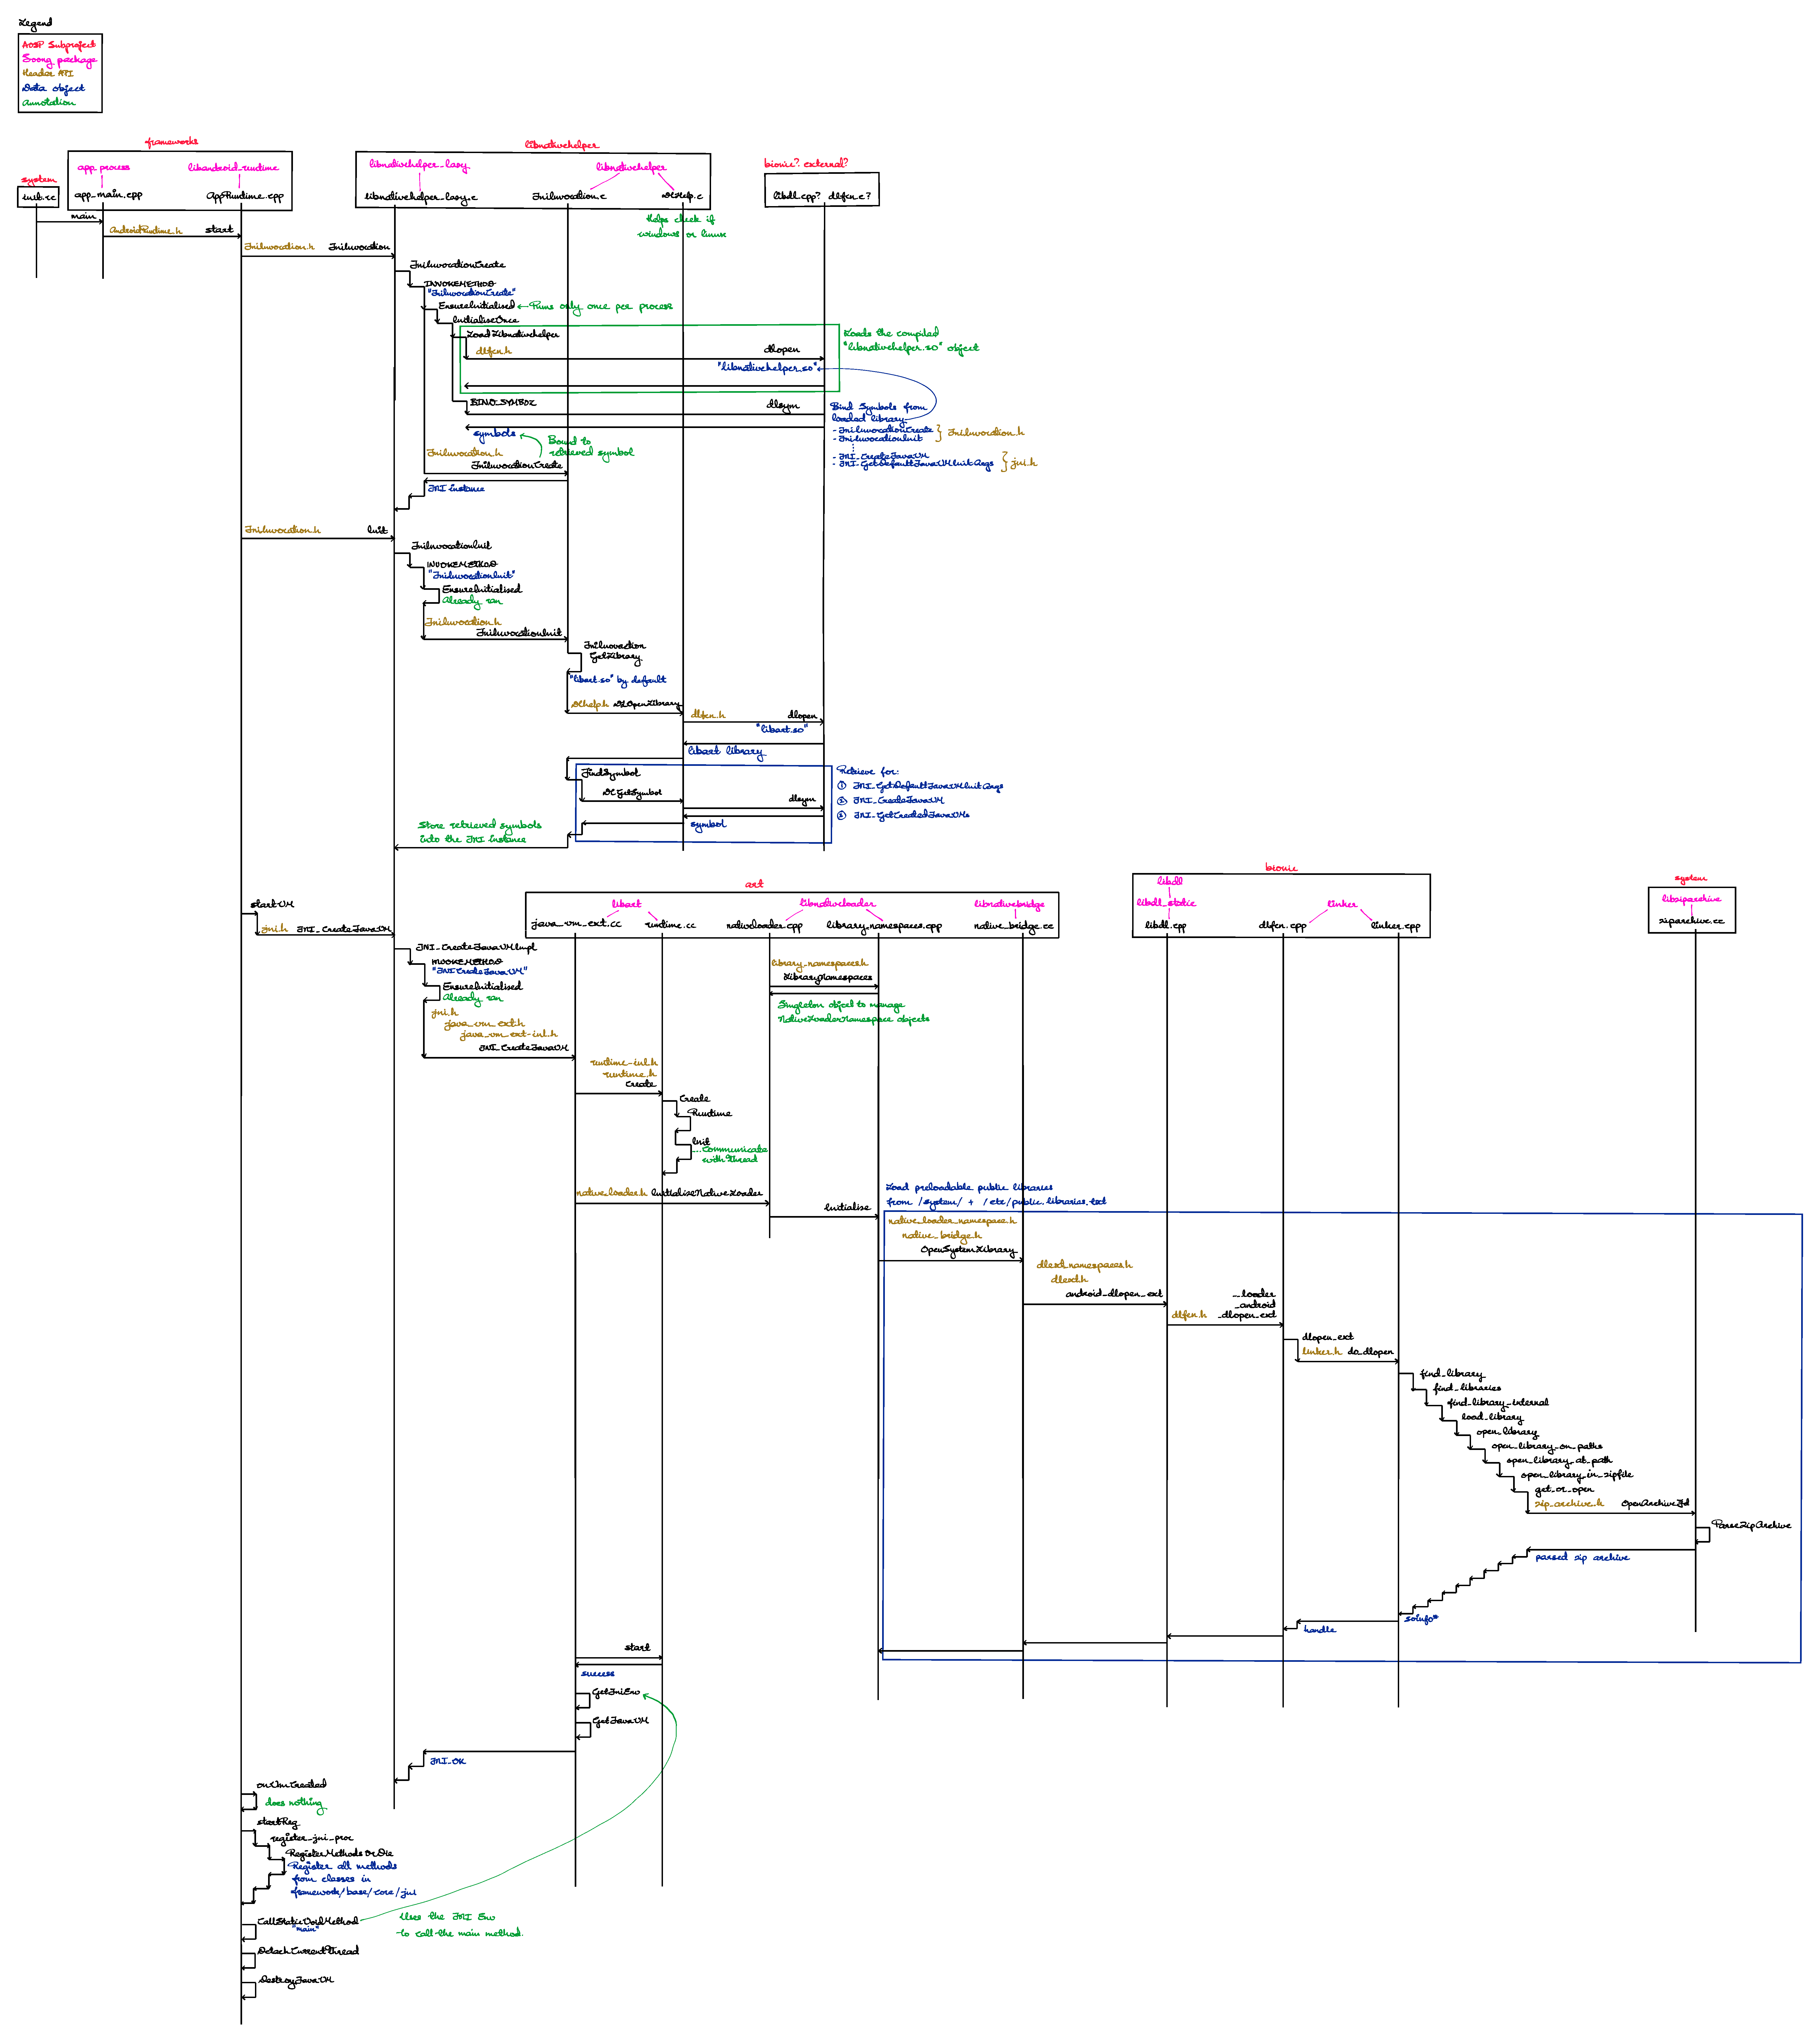
\includepdf[pages=-, scale=.95,pagecommand={}]{entries/2024/01/01/art.pdf}

% \begin{itemize}
% \item \textbf{Domain.} The context of the process that is acting upon something.
% \item \textbf{Type.} The context of the resource on which the process is acting.
% \item \textbf{Class.} The object class of the resource (e.g. \textit{file} or \textit{socket}).
% \item \textbf{Permissions.} The permissions that are allowed given the \textit{domain}, \textit{type} and \textit{class}.
% \end{itemize}

% SELinux rule syntax:
% \begin{lstlisting}
% allow <domain> <type>:<class> { <permissions> };
% \end{lstlisting}

% \subsubsection{Decoding Permission Denial Message}

% Message:
% \begin{lstlisting}
% type=AVC msg=audit(1363289005.532:184): avc:  denied  { read } for  pid=29199 comm="Trace" 
% name="online" dev="sysfs" ino=30 scontext=staff_u:staff_r:googletalk_plugin_t 
% tcontext=system_u:object_r:sysfs_t tclass=file
% \end{lstlisting}

% \begin{longtable}{p{.15\linewidth}p{.15\linewidth}p{.65\linewidth}} 
% \toprule
% Log part & Name & Description \\
% \midrule
% \endhead

% \texttt{type=AVC}
% &Log type
% &Only in the \texttt{audit.log} file; it informs the user what kind of audit log type this is. 
% \\

% \texttt{msg=audit(1363289005.532:184)}
% &Timestamp
% &Timestamp in seconds since epoch, meaning the number of seconds since January 1st, 1970. You can convert this to a more human readable format using date -d @ followed by the number, like so: \texttt{date -d @1363292159.532}.
% \\

% \texttt{avc:}
% &Log type (again)
% &
% \\

% \texttt{ino=30}
% &inode number
% &The inode number of the target file. In this case, since we know it is on the \texttt{sysfs} file system, we can look for this file using: \texttt{find /sys -xdev -inum 30}
% \\

% \texttt{scontent=staff\_u:staff\_r:googletalk\_plugin\_t}
% &Source context
% &The security context of the process (the domain)
% \\

% \texttt{tcontext=system\_u:object\_r:sysfs\_t}
% &Target context
% &The security context of the target resource (in this case the file)
% \\

% \texttt{tclass=file}
% &Target class
% &The class of the target.
% \\

% \midrule
% \caption{Permission Denied Syntax} 
% \label{tab:permissiondeniedsyntax}
% \end{longtable}


% \subsubsection{SELinux Architecture}

% SELinux consists of four main components: object managers (OM), access vector cache (AVC), security server, and security policy as show below:
% \begin{figure}[H]
%     \centering
%     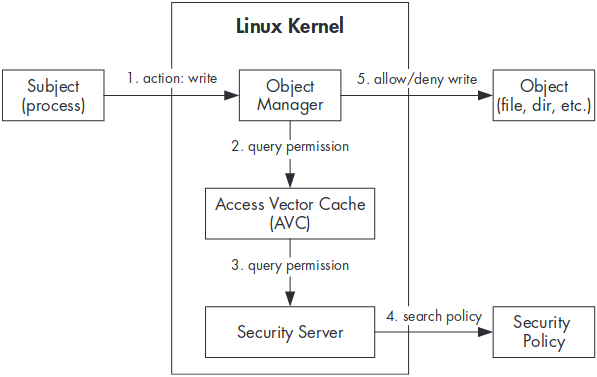
\includegraphics[width=.85\linewidth]{entries/2023/12/10/selinux.png}
%     \caption{SELinux Components}
%     \label{fig:selinux}
% \end{figure}
